\section{The Aharonov-Bohm Effect}
\subsection{Hamiltonian}
Since the magnetic flux is only through the middle of the ring, there is no magnetic field (onlt a potential) on the ring itself, therefore the hamiltonian won't include an element for the interaction of the spin and the magnetic field. Therefore
\begin{equation}
	H = \frac{1}{2m}\ins{\vec{p}-e\vec{A}}^2
\end{equation}
inserting the vector potential we have
\begin{equation}
	H = \frac{1}{2m}\ins{\vec{p}-\frac{e\Phi}{L}}^2
\end{equation}
we can constrain the momentum element because we know the particle is on the ring, therefore
\begin{equation}
	\vec{p} = -\frac{\hbar}{i}\del_x = -\frac{\hbar}{iR}\del_\theta
\end{equation}
so the hamiltonian is
\begin{equation}
	H = \frac{\hbar^2}{2mR^2}\ins{-i\del_\theta+\frac{e\Phi}{2\pi\hbar}}^2
\end{equation}
and the Schrodinger equation is
\begin{equation}
	i\hbar\del_t\psi = \frac{\hbar^2}{2mR^2}\ins{-i\del_\theta+\frac{e\Phi}{2\pi\hbar}}^2\psi
\end{equation}
\subsection{Setting X}
I already did this in the previous subsection.\ x is defined in \(\left[0,L\right]\). We can define the basic flux unit \(\Phi_0 = 2\pi\hbar/e\) and find
\begin{equation}
	H = \frac{\hbar^2}{2mR^2}\ins{-i\del_\theta+\frac{\Phi}{\Phi_0}}^2
\end{equation}
\subsection{Energy Spectrum}
We'll perform a gauge transform, defining \(\phi = \frac{\Phi}{\Phi_0}\)
\begin{equation}
	\psi(\theta) = e^{-i\phi\theta}\chi(\theta)
\end{equation}
Which gives us
\begin{align}
	\ins{-i\del_\theta+\phi} e^{-i\phi\theta}\chi(\theta) &= \ins{-\phi\chi(\theta) - i\chi'(\theta)+\phi\chi(\theta)}e^{-i\phi\theta} \\
	&= -ie^{-i\phi\theta}\chi'(\theta)
\end{align}
therefore
\begin{equation}
	\ins{-i\del_\theta+\phi} \psi(\theta) = -ie^{-i\phi\theta}\del_\theta \chi(\theta)
\end{equation}
if we apply the operator again
\begin{equation}
	\ins{-i\del_\theta+\phi}^2 \psi(\theta) = e^{-i\phi\theta}\ins{-i\del_\theta}^2 \chi(\theta)
\end{equation}
so the Schrodinger equation becomes
\begin{equation}
	\frac{\hbar^2}{2mR^2}\ins{-i\del_\theta}^2 \chi(\theta) = E\chi(\theta)
\end{equation}
which is the Schrodinger equation for a free particle. This also means \(\chi\) has a solution of the form
\begin{equation}
	\chi(\theta) = e^{ik\theta}
\end{equation}
Next we consider the boundary conditions which changed due to the gauge transform. We know the problem has periodic boundary conditions, therefore
\begin{equation}
	e^{-i\phi\theta}\chi(\theta) = e^{-i\phi(\theta+2\pi)}\chi(\theta+2\pi)
\end{equation}
rearranging
\begin{equation}
	\chi(\theta) = e^{-2\pi i \phi}\chi(\theta+2\pi)
\end{equation}
inserting the solution ansatz
\begin{equation}
	e^{ik\theta} = e^{-2\pi i \phi} e^{ik\ins{\theta+2\pi}} \implies e^{2\pi i \phi} = e^{2\pi i k}
\end{equation}
therefore
\begin{equation}
	k = n + \phi \qquad n \in \mathds{N}
\end{equation}
and this gives us the energy spectrum
\begin{equation}\label{energylevels}
	E_n = \frac{\hbar^2}{2mR^2}\ins{n+\phi}^2
\end{equation}
as needed.
\subsection{Gauge transform}
I already showed the energy spectrum in the previous subsection.
\newpage
\subsection{Drawing the Spectrum}
\begin{figure}[!htb]
	\centering
	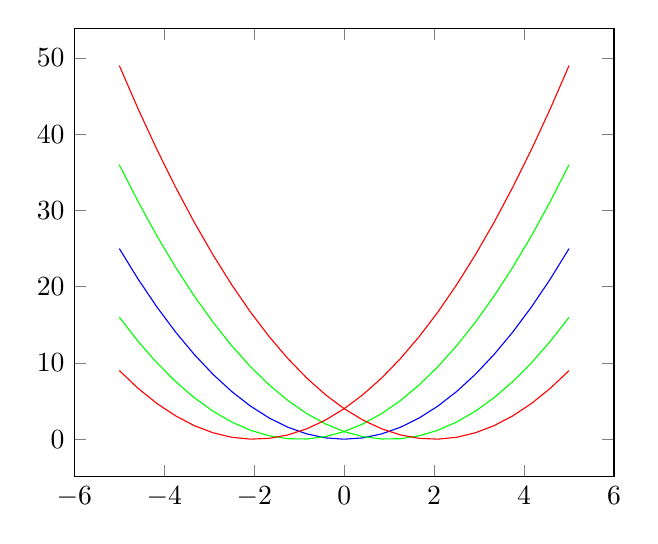
\begin{tikzpicture}
		\begin{axis}[domain=-5:5]
			\addplot[blue, no marks]{x^2};
			\addplot[green, no marks]{(1+x)^2};
			\addplot[green, no marks]{(-1+x)^2};
			\addplot[red, no marks]{(2+x)^2};
			\addplot[red, no marks]{(-2+x)^2};
		\end{axis}
	\end{tikzpicture}
	\caption{The energy spectrum described by equation~\ref{energylevels} for \(n=0,\pm 1, \pm 2\) marked by blue, green, and red respectively, in multiples of \(\frac{\hbar^2}{2mR^2}\). I drew this figure using tikz.}
\end{figure}
\subsection{Reduced Representation}
\begin{figure}[!htb]
	\centering
	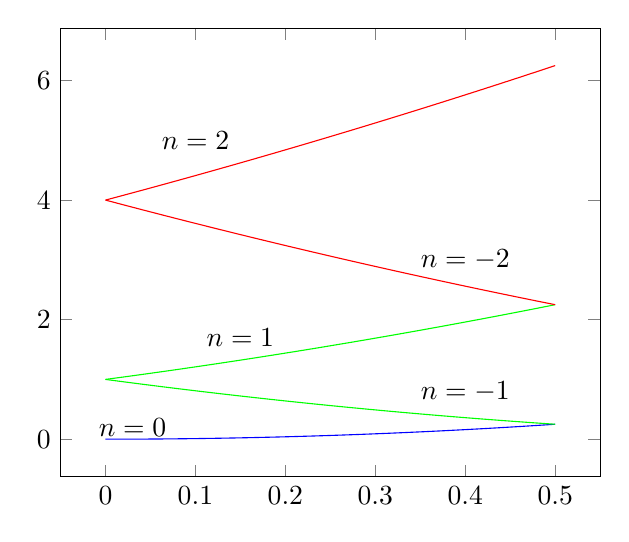
\begin{tikzpicture}
		\begin{axis}[domain=0:0.5]
			\addplot[blue, no marks]{x^2};
			\node at (axis cs:0.03,0.2){\(n=0\)};
			\addplot[green, no marks]{(1+x)^2};
			\node at (axis cs:0.15,1.7){\(n=1\)};
			\addplot[green, no marks]{(-1+x)^2};
			\node at (axis cs:0.4,0.8){\(n=-1\)};
			\addplot[red, no marks]{(2+x)^2};
			\node at (axis cs:0.1,5){\(n=2\)};
			\addplot[red, no marks]{(-2+x)^2};
			\node at (axis cs:0.4,3){\(n=-2\)};
		\end{axis}
	\end{tikzpicture}
	\caption{The energy spectrum described by equation~\ref{energylevels} for \(n=0,\pm 1, \pm 2\) marked by blue, green, and red respectively, in multiples of \(\frac{\hbar^2}{2mR^2}\), in the domain \(0-0.5\). I drew this figure using tikz.}
\end{figure}

The reason we can reduce our focus on just \(0-0.5\) is that the energy spectrum is periodic in terms of \(\phi\). Since it depends on two numbers, one continuous (\(\phi\)) and one discrete (\(n\)), any value of \(\phi\) over \(0.5\) is the same as taking a \(\phi\) less than one half and adding a negative \(n\).
\subsection{Odd and Even Energy Spectrum}
We'll define
\begin{equation}
	n(p) = \begin{cases}
		\frac{p}{2} & p \text{ is even} \\
		-\frac{p+1}{2} & p \text{ is odd}
	\end{cases}
\end{equation}
and insert it into equation~\ref{energylevels}
\begin{equation}
	E_p = \frac{\hbar^2}{2mR^2}\begin{cases}
		\ins{\frac{p}{2}+\phi}^2 & p \text{ is even} \\
		\ins{-\frac{p+1}{2}+\phi}^2 & p \text{ is odd}
	\end{cases}
\end{equation}
but we can take out the minus sign from the parentheses and have
\begin{equation}
	E_p = \frac{\hbar^2}{2mR^2}\begin{cases}
		\ins{\frac{p}{2}+\phi}^2 & p \text{ is even} \\
		\ins{\frac{p+1}{2}-\phi}^2 & p \text{ is odd}
	\end{cases}
\end{equation}
because \(-1^2=1\).
\subsection{Degeneracy}
\subsubsection{For \(\phi=0\)}
The energy level for \(p=0\) will have a degeneracy of 1, the rest will have a degeneracy of 2.
\subsubsection{For \(\phi=\frac{1}{2}\)}
If we insert \(\phi=\frac{1}{2}\) into the energy levels we find
\begin{equation}
	E_p = \frac{\hbar^2}{2mR^2}\begin{cases}
		\ins{\frac{p+1}{2}}^2 & p \text{ is even} \\
		\ins{\frac{p}{2}}^2 & p \text{ is odd}
	\end{cases}
\end{equation}
which is identical to the case \(\phi=0\)
\subsubsection{For \(0<\phi<\frac{1}{2}\)}
All energy levels will have a degeneracy of 1, because no two additions of p and \(\phi\) will match for different \(p\)s.